\section{Breakdown of costs}\label{app:cost-nodes}

\begin{figure}[H]
    \centering
    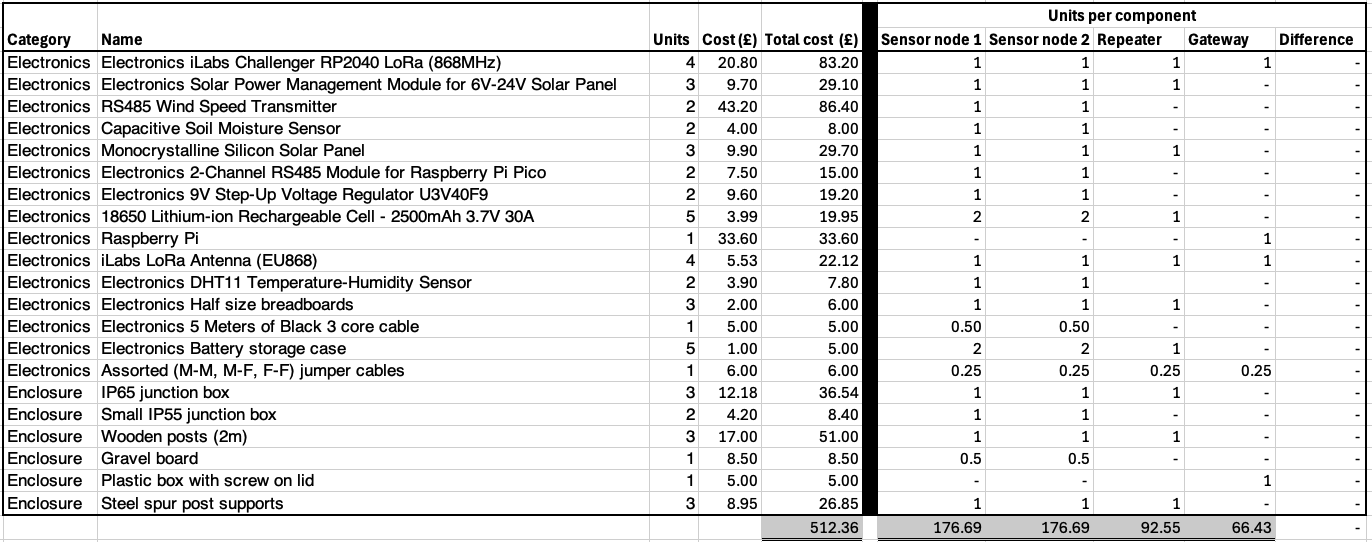
\includegraphics[width=1\textwidth]{contents/appendix/fig5/table.jpg}
    \caption{Table of component costs}
    \label{fig:cost-table}
\end{figure}

\begin{figure}[H]
    \centering
    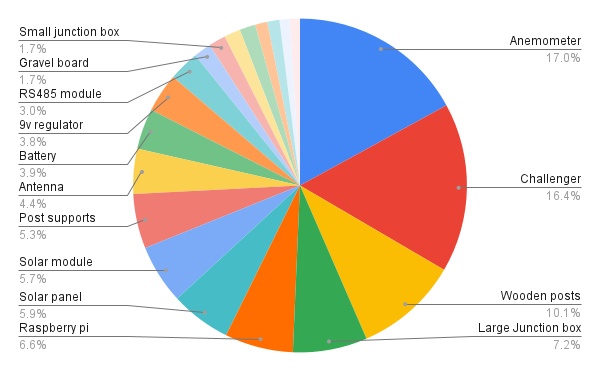
\includegraphics[width=0.8\textwidth]{contents/appendix/fig5/chart.png}
    \caption{Chart to visualise relative cost of components}
    \label{fig:cost-chart}
\end{figure}

\section{Interview excerpt with Small Brook Farms
owners}\label{sec:small-brook-interview}

Interviewer: So you would need a weather station to observe very local weather,
I expect. What you're saying is that the BBC website weather is not necessarily
relevant to you?

Speaker 1: No, No , so there's another site which is in Sanford and we can have
conversations - we're what? - 5 miles apart 10 miles? 

Speaker 2: Yeah. So the other side of that hill there like a mile away you get a
different sort of weather, but even on this side of the [apple orchard] as
opposed to that side of the [apple orchard] like the wind can be less than
whatever else, its very localised. But you know you if you then go on that side
of the valley, it doesn't rain on this side. So like to be actually useful,
yeah, [weather monitoring] sort of has to be [based on] the farm.

Source: Transcript no.28 of site visit from DECIDE sharepoint (9 May 2025)

\section{Battery cost assumptions}\label{app:battery-assumptions}
\begin{itemize}
  \item \textbf{Agriscanner Network:} Replace 5 (2 per sensor node, 1 for
  repeater) Li-ion batteries every 3 years at a cost of \pounds{}20
  \(\Rightarrow\) \(\approx\)\,\pounds{}7 per annum.
  \item \textbf{SenseCAP S2120:} Three AA batteries per node, replaced twice a
  year (total 12 batteries) \(\approx\)\,\pounds{}10 per annum.
  \item \textbf{Decentlab Eleven Parameter:} Two C batteries per node, replaced
  four times per year (total 16 batteries) \(\approx\)\,\pounds{}30 per annum.
  \item \textbf{HOBO weather station kit:} Replace lead-acid for each node
  battery every 4 years at a cost of \pounds{}80 \(\Rightarrow\)
  \(\approx\)\,\pounds{}20 per annum.
\end{itemize}

\section{System usability survey}\label{app:sus-survey}

\begin{figure}[H]
    \centering
    
\includegraphics[width=0.9\textwidth]{contents/appendix/fig5/sus_survey.png}
    \caption{SUS survey wording}
    \label{fig:survey-wording}
\end{figure}

List of tasks for users:

\begin{enumerate}\label{list-of-tasks}
  \item To the nearest degree, what was Node 2's temperature at 14:00 18 August
  2025?
  \item To the nearest 1\,m/s, what was Node 1's gust speed at 13:00 26 August
  2025?
  \item Go to wind speed and change the graph to compare mode. What colour is
  Node 2 gusts represented by?
  \item What is the forecast for humidity at 06:00 tomorrow for Node 1?
\end{enumerate}

\section{Additional SUS materials}\label{app:correlation-sus}

\begin{figure}[H]
    \centering
    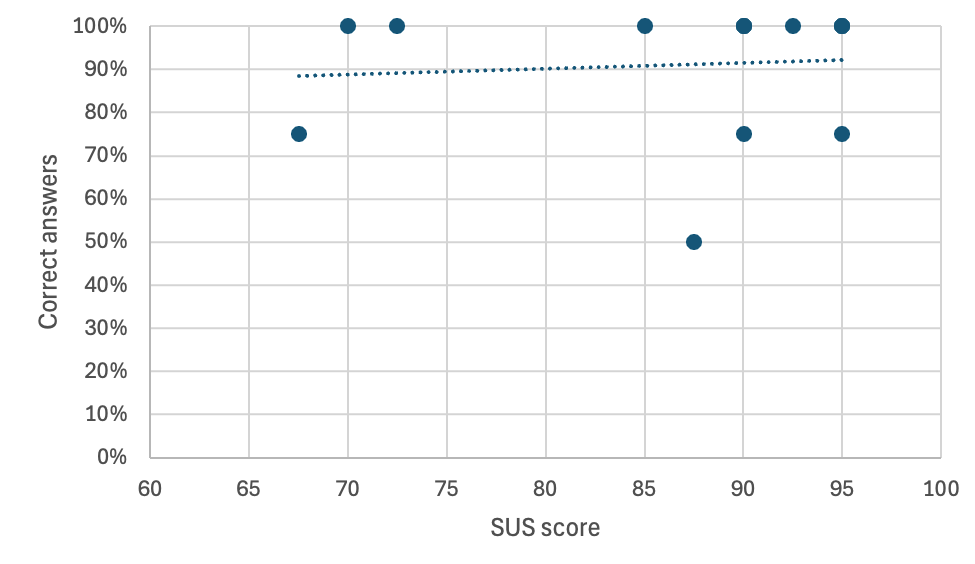
\includegraphics[width=0.9\textwidth]{contents/appendix/fig5/answer-sus-correlation.png}
    \caption{Graph to show SUS score vs percent of correct answers ($R^2 = 0.0066$)}
    \label{fig:sus-correlation}
\end{figure}

\begin{table}[ht]
  \centering
  \begin{tabular}{r r r r}
    \hline
    responder\_num & sus\_score & correct\_answers & type\\
    \hline
    1  &  90.0  & 75\%  & desktop\\
    2  &  92.5  & 100\% & mobile\\
    3  &  95.0  & 100\% & mobile\\
    4  &  70.0  & 100\% & desktop\\
    5  &  90.0  & 100\% & mobile\\
    6  &  90.0  & 100\% & desktop\\
    7  &  87.5  & 50\%  & desktop\\
    8  &  95.0  & 100\% & mobile\\
    9  &  95.0  & 75\%  & mobile\\
    10 &  95.0  & 100\% & desktop\\
    11 &  72.5  & 100\% & desktop\\
    12 &  67.5  & 75\%  & mobile\\
    13 & 100.0  & 100\% & mobile\\
    14 &  90.0  & 100\% & mobile\\
    15 &  85.0  & 100\% & desktop\\
    \hline
  \end{tabular}
  \caption{Raw SUS scores and correct answer percentage from survey}
  \label{tab:raw-sus}
\end{table}

% Requires: \usepackage{float} Also requires: \usepackage{amsmath}
\begin{figure}[H]
  \centering
  \begin{minipage}{0.9\textwidth}
    \begin{quote}
    ``I found it very hard to get to a specific time on the graph - the
    granularity of the cursor moving seemed to make it hard to choose my time -
    I ended up with 14:01 for the first question as I couldn't get the cursor to
    stay at 14:00. But as a weather nerd I loved it.''
    \end{quote}
 \vspace{8pt}
    \begin{quote}
    ``I found it annoying having to click to get to the required date. Also I
    don't understand from the website alone what the project is about or where
    the data is from - maybe an about page would be nice :)''
    \end{quote}
 \vspace{8pt}
    \begin{quote}
    ``Sorry wasn’t sure where the compare graph is but the website looked really
    nice!''
    \end{quote}
  \end{minipage}
  \caption{Feedback from participants with lower SUS scores}
  \label{fig:low-sus-feedback}
\end{figure}

\begin{figure}[H]
  \centering
  \begin{minipage}{0.9\textwidth}
    \begin{quote}
    "The soil moisture readings surprised me - I expected them to go up with
    rain (increased moisture) but they went down.  I think this is
    counter-intuitive and there should either be some explanation of the what
    the measurements mean, or preferably there should be an option to convert to
    a more human understandable description like very dry/dry/slightly
    moist.../wet/very wet/saturated"
    \end{quote}
 \vspace{8pt}
    \begin{quote}
    "When selecting the date (specifically when clicking the arrows to move
    forwards and backwards in time) it would be useful to have a calendar
    display to travel to past dates quicker."
    \end{quote}
 \vspace{8pt}
    \begin{quote}
    "Extra features: - Date picker instead of having to navigate past each day -
    Export feature to export data in bulk (e.g. to a csv) - Ability to select a
    time period (specific dates) instead of just a day view"
    \end{quote}
 \vspace{8pt}
    \begin{quote}
    "I think when switching dates, it should support selecting a date from the
    calendar rather than only moving forward or backward to the nearest dates."
    \end{quote}
 \vspace{8pt}
    \begin{quote}
    "Being able to navigate directly between measurements (e.g. temp, humidity
    etc.) while on [sic]"
    \end{quote}
 \vspace{8pt}
    \begin{quote}
    "Finding the "compare" option was the hardest part. But didn't take long." 
    \end{quote}
 \vspace{8pt}
    \begin{quote}
    "Great website- simple layout and easy to use!"
    \end{quote}
 \vspace{8pt}
    \begin{quote}
    "No bugs seen, but on wind graph some of the y axis text was slightly cut
    off on my screen. I'm on a laptop"
    \end{quote}
  \end{minipage}
  \caption{Feedback from participants with higher SUS scores}
  \label{fig:high-sus-feedback}
\end{figure}

\begin{figure}[H]
  \makebox[\textwidth][r]{ \fbox{
      \begin{minipage}[c][8cm][c]{0.85\textwidth}
        \raggedright

        Both the Mann Whitney U and Wilcoxon Signed Rank test were selected for
        this data because the SUS score is derived from Likert items. Likert
        items are ordinal (e.g. strongly disagree) and so nonparametric
        statistical testing is typically preferred
        \cite{bobbitt_mann-whitney_2022}\vspace{8pt}

    The Mann Whitney U statistical test score was calculated in an Excel sheet I
    made using the procedure described in \cite{bobbitt_mann-whitney_2022} and
    the result cross-verified using the website in \cite{socscistats} which is
    also the source of the p-value. Results: U = 13.5, critical value = 10
    p=0.10524. Parameters: two-tailed, 0.05 significance\vspace{8pt}
    
    Due to the complexity of calculating it, the one-sample Wilcoxon Signed Rank
    Test score was calculated in Excel using a modified template from the source
    in \cite{peterstatistics_wilcoxon_2025} and cross-verified with the website
    in \cite{statsBlue}. Results: \(W^{+}=119\) z = 3.3361, critical value =
    1.6449 Parameters: right-tailed, 0.05 significance \end{minipage} } }
  \caption{Note on statistical testing}
  \label{fig:appendix-note-1}
\end{figure}

% \section{Nielsen's nine usability heuristics
% \cite{nielsen1990heuristic}}\label{app:usability-heuristics}

% \begin{itemize}
%   \item Simple and natural dialogue
%   \item Speak the user's language
%   \item Minimize user memory load
%   \item Be consistent
%   \item Provide feedback
%   \item Provide clearly marked exits
%   \item Provide shortcuts
%   \item Good error messages
%   \item Prevent errors
% \end{itemize}


\section{How LoRa works}\label{app:lora-explained}

As this paper is not a technical study of radio communication I will opt for a
brief summary of the principles behind LoRa. With this in mind I have based much
of the information from the excellent video lecture in \cite{visualelectric2021}
that itself draws upon the paper in \cite{vangelista2017}.

The reason LoRa modulation is different to traditional modulation techniques is
the use of a "chirp" as the key to transmitting packets. A more traditional
technique might involve a frequency shift key; that is a single frequency
represents several bits. These unique frequencies are called symbols as they
represent data, like letters in the alphabet. In the below graph we see three
simplified symbols that represent binary values, the combination of these
symbols makes a packet:

\begin{figure}[H]
  \centering
  % left image
  \begin{minipage}{0.48\textwidth}
    \centering
    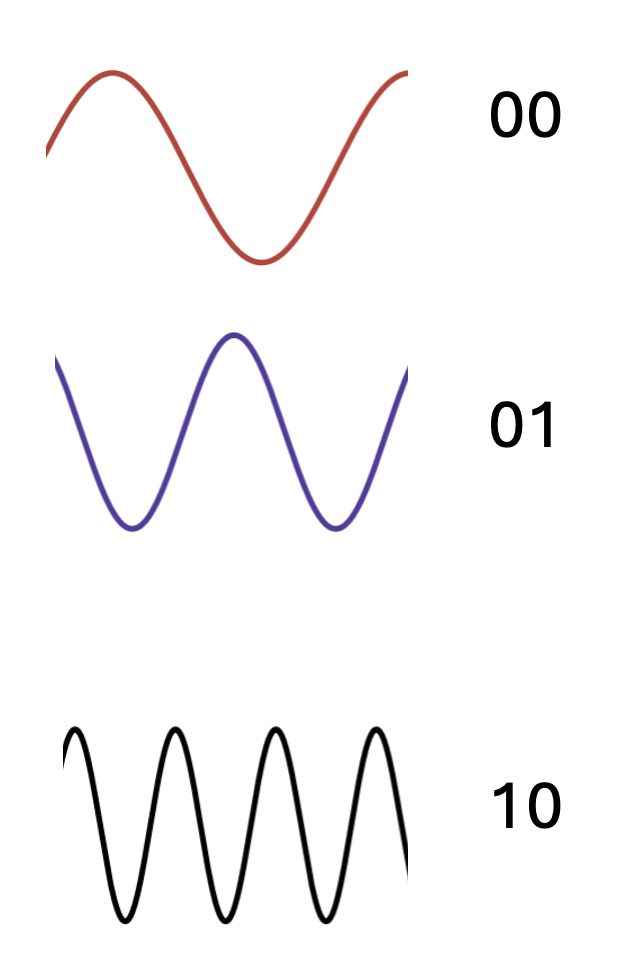
\includegraphics[width=0.4\linewidth]{contents/part-1/fig1/frequencysymbols.png}
    \\[4pt]
    {\small (a) Frequency shift symbols} \end{minipage}\hfill
  % right image
  \begin{minipage}{0.48\textwidth}
    \centering
    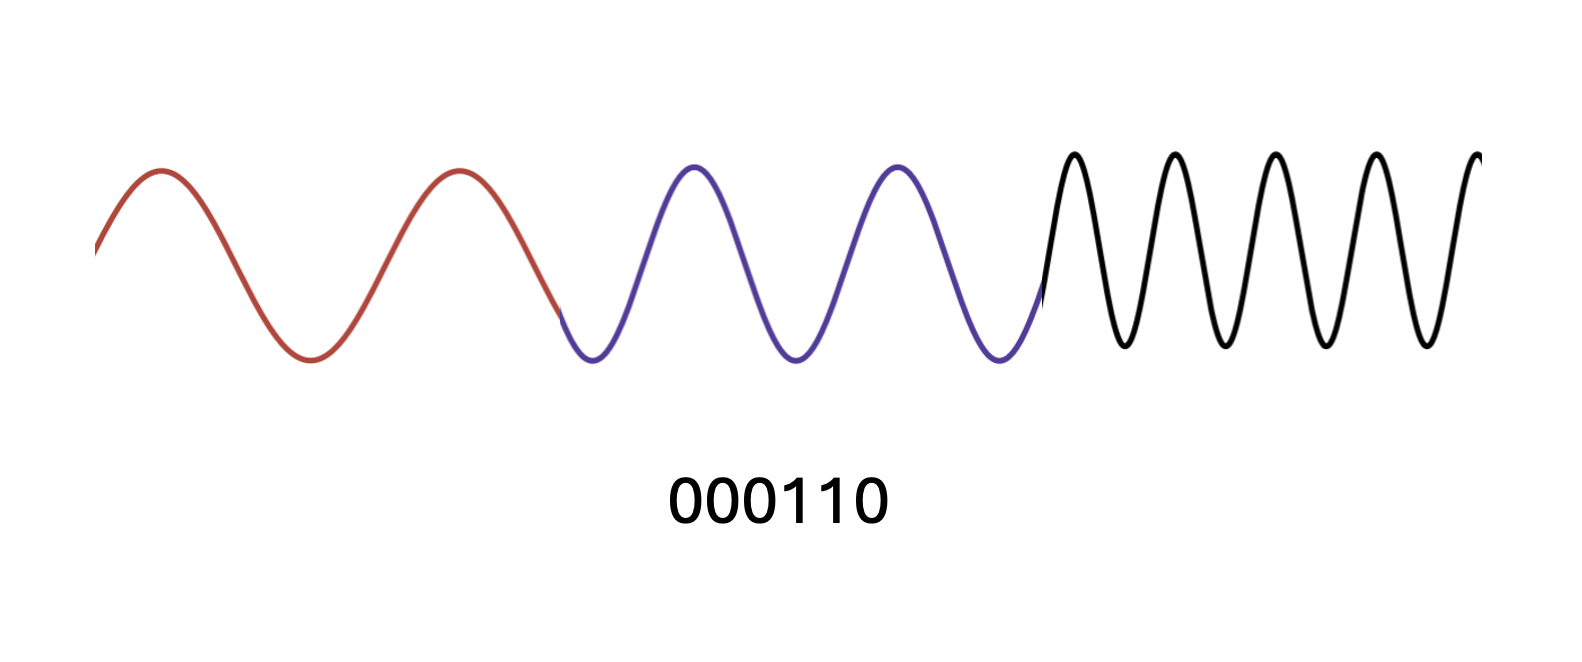
\includegraphics[width=1\linewidth]{contents/part-1/fig1/packet.png}
    \\[4pt]
    {\small (b) Packet}
  \end{minipage}
  \caption{ Traditional radio modulation with frequency symbols}
  \label{fig:freq-and-packet}
\end{figure}

In traditional modulation, symbols always have flat unchanging frequency (as can
be seen from the fact the wave separation never changes). LoRa symbols instead
have changing frequencies that have a waveform like the below.

\begin{figure}[H]
    \centering
    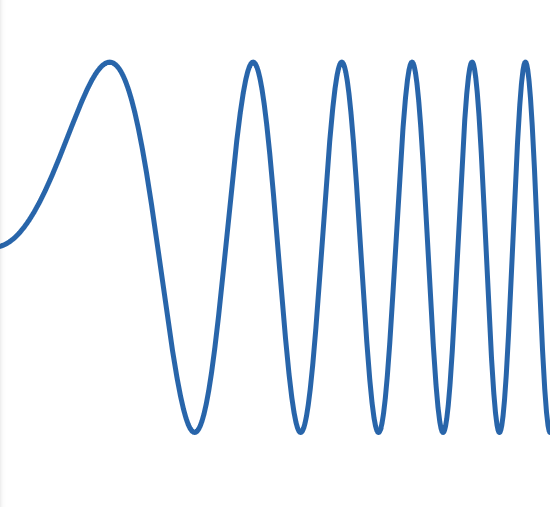
\includegraphics[width=0.15\textwidth]{contents/part-1/fig1/lorawavelength.png}
    \caption{LoRa symbol showing changing frequency ("Up-chirp")}
    \label{fig:lora-wave}
\end{figure}

This change in frequency is what gives the wave form the name "chirp". If
traditional frequency symbols were thought of a sound they would be similar to
morse code beeps while LoRa would be more similar to siren or \textit{chirp}ing
bird. LoRa has both rising and falling chirps (up-chirps and down-chirps).

Different LoRa symbols are then distinguished by the point in time of a
discontinuity. LoRa symbols are always delivered over a known length of time, so
different symbols include a reset back to the starting frequency at a different
point in time.

A way to graphically show this discontinuity in LoRa and compare it to frequency
shift modulation is by using instantaneous frequency graphs:

\begin{figure}[H]
  \centering
  % left image
  \begin{minipage}{0.48\textwidth}
    \centering
    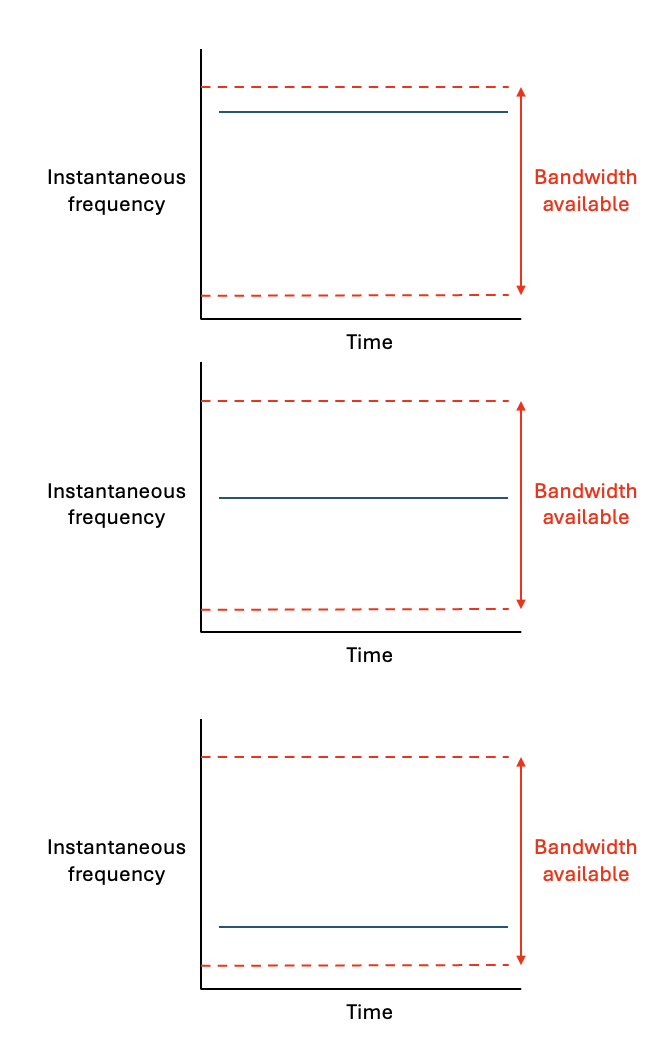
\includegraphics[width=0.9\linewidth]{contents/part-1/fig1/traditional-wavechart.png}
    \\[4pt]
    {\small (a) Frequency shift symbols} \end{minipage}\hfill
  % right image
  \begin{minipage}{0.48\textwidth}
    \centering
    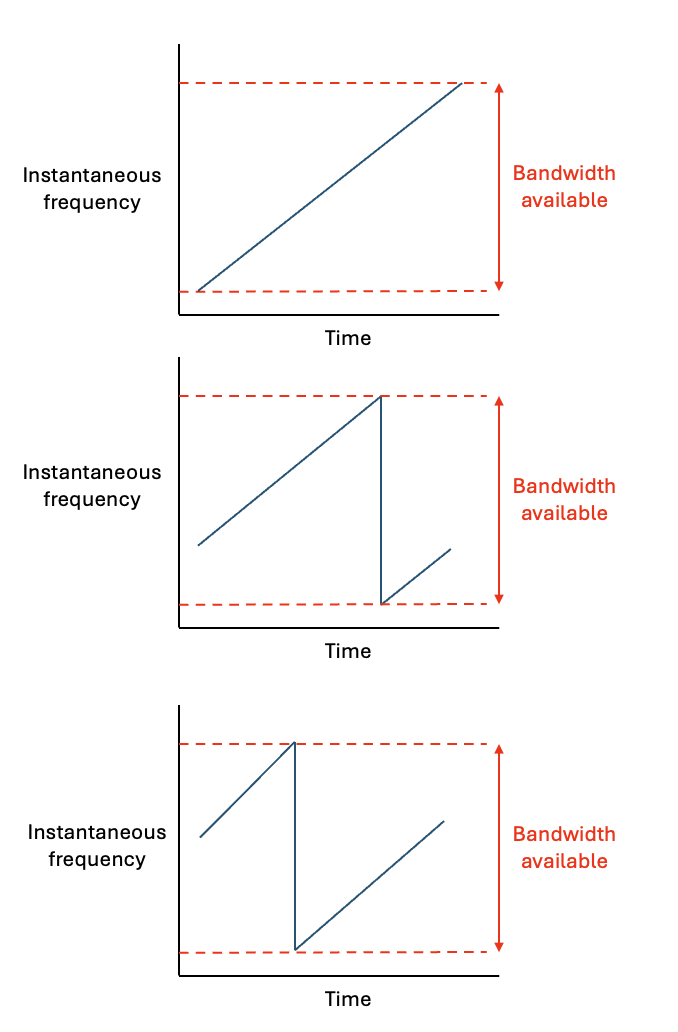
\includegraphics[width=0.9\linewidth]{contents/part-1/fig1/lora-wavechart.png}
    \\[4pt]
    {\small (b) LoRa symbols, note shifting discontinuity}
  \end{minipage}
  \caption{ Comparison of frequency shift and LoRa modulation }
  \label{fig:freq-vs-lora}
\end{figure}

Once these symbols hit the receiver, the receiver must work out which symbol it
was. In frequency shift modulation this is achieved by performing a correlation
test against every symbol received. However this is computationally difficult
and requires a low signal-to-noise ratio to work effectively. The benefit of
chirps is that due to a mathematical transformation that will not be further
discussed (Fast Fourier transform), the correlation can be computed much more
easily and with less powerful hardware.


\section{IoT enabling technologies} \label{app:enabling-tech}

This supplementary section lists the key technological developments that have
are contributed to the viability of my project.

\begin{enumerate}
  \item Efficiency improvements in microchips - breakthroughs in microchip
  fabrication have led to smaller more efficient chips with improved
  performance.
  \item Lithium-Ion batteries improvements - continuous improvements in the
  energy density of lithium-ion batteries has made it possible to power devices
  for long periods without mains power.
  \item Low-power long-range radio - new radio communication techniques such as
  LoRa allow for data transmission over several kilometres using a fraction of
  the power required by traditional mobile or Wi-Fi technologies.
  \item Affordability of solar panels - since 1970 the price of solar panels has
  decreased to 1/500th of its original cost \cite{economist2024} making solar a
  viable power source for IoT systems.
  \item Growth of hobbyist embedded systems - since the release of accessible
  platforms such as Arduino in 2005, the growth of hobby level embedded systems
  has lowered the barrier to entry to create IoT systems.
  \item Accessible cloud computing and hosting - Cheap and available web hosting
  has allowed application level systems to be more easily developed.
\end{enumerate}

\section{CircuitPython sensor node 1 code example}\label{app:sensor-code}

\begin{multicols}{2}
\begin{lstlisting}
import time
import board
import busio
import digitalio
import adafruit_rfm9x
import adafruit_dht
import analogio


DEVICE_ID = 1
RADIO_FREQ_MHZ = 868.0
WIND_REQUEST = bytes([0x02, 0x03, 0x00, 0x00, 0x00, 0x01, 0x84, 0x39])

# Initialise LORA radio and settings
try:
    spi = busio.SPI(board.RFM95W_SCK, MOSI=board.RFM95W_SDO, MISO=board.RFM95W_SDI)
    cs  = digitalio.DigitalInOut(board.RFM95W_CS)
    rst = digitalio.DigitalInOut(board.RFM95W_RST)
    rfm9x = adafruit_rfm9x.RFM9x(spi, cs, rst, RADIO_FREQ_MHZ)

    rfm9x.tx_power = 13
    rfm9x.spreading_factor = 7
    rfm9x.signal_bandwidth = 125_000
    rfm9x.coding_rate      = 5
    rfm9x.enable_crc       = True
    rfm9x.implicit         = False

except Exception as e:
    rfm9x = None
    print("ERR: Lora module", e)
    
# Initialise UART and settings    
try:
    uart = busio.UART(tx=board.GP16, rx=board.GP17, baudrate=9600, timeout=0.2)
except Exception as e:
    uart = None
    print("ERR: UART", e)
    
# Initialise the soil moisture sensor    
try:    
    moisture_pin = analogio.AnalogIn(board.A0)
except Exception as e:
    moisture_pin = None
    print("ERR: moisture pin", e)

# Initialise DHT11 temperature humidity sensor
try:
    dht_device = adafruit_dht.DHT11(board.A1)
except Exception as e:
    dht_device = None
    print("ERR: dht11", e)
    
# Returns raw soil moisture reading
def get_raw_moisture(pin):
    try:
        raw = pin.value   
        return raw
    except:
        return None

# Returns wind speed sensor using MODBUS protocol
def get_wind_speed():
    if uart:
        try:
            uart.write(WIND_REQUEST)
            time.sleep(0.2)
            response = uart.read(16)
            if response:
                if len(response) >= 5 and response[0] == 0x02 and response[1] == 0x03:
                    value_raw = response[3] << 8 | response[4]
                    return value_raw / 10.0
                else:
                    print("Bad format error")
                    return None
            else:
                print("No response error")
                return None
        except:
            print("Unknown error")
            return None
    print("Bad UART error")
    return None

def find_err(value):
    if value is None:
        return "ERR"
    else:
        return value

counter = 0

while True:
    
    t_sum = h_sum = w_sum = 0.0
    s_sum = 0
    t_n = h_n = s_n = w_n = 0
    min_counter = 0
    w_max = 0
    
    while min_counter < 10:
        if dht_device:
            try:
                t_reading = dht_device.temperature
                if t_reading is not None:
                    t_sum += float(t_reading)
                    t_n += 1
            except Exception:
                pass
            try:
                h_reading = dht_device.humidity
                if h_reading is not None:
                    h_sum += float(h_reading)
                    h_n += 1
            except Exception:
                pass
        s_reading = get_raw_moisture(moisture_pin)
        
        if s_reading is not None:
            s_sum += s_reading
            s_n += 1
            
        w_reading = get_wind_speed()
        
        if w_reading is not None:
            w_sum += float(w_reading)
            w_n += 1
            if w_reading > w_max:
                w_max = w_reading
        
        min_counter += 1
        time.sleep(6)
        
        
    if t_n != 0:    
        t_avg = t_sum/t_n
    else:
        t_avg = None
    if h_n != 0:    
        h_avg = h_sum/h_n
    else:
        h_avg = None
    if s_n != 0:    
        s_avg = s_sum/s_n
    else:
        s_avg = None
    if w_n != 0:
        w_avg = w_sum/w_n
    else:
        w_avg = None
        w_max = None
    
    payload = f"{DEVICE_ID},{find_err(t_avg)},{find_err(h_avg)},{find_err(s_avg)},{find_err(w_avg)}, {find_err(w_max)},{counter}"
    try:
        rfm9x.send(payload.encode("utf-8"))
        print(f"Sent packet {payload}")
    except Exception as e:
        print("Failed to send packet: ", e)

    counter += 1
\end{lstlisting}
\end{multicols}

\section{Typescript API endpoint code for node data
insert}\label{app:api-endpoint}
\begin{multicols}{2}
\begin{lstlisting}
app.post('/api/database/insert-node-data', async (req: Request, res: Response) => {
  const {
    device_id,
    packet_id,
    temperature,
    humidity,
    soil_moisture,
    wind_speed,
    gust_speed,
    rssi0,
    rssi1,
    snr0,
    snr1,
  } = req.body;

  try {
    const query = `INSERT INTO node_data 
      (node_deployment_id, farm_id, packet_id, temperature, humidity, 
      soil_moisture, wind_speed, gust_speed, rssi0, rssi1, snr0, snr1, node_name)
      VALUES (
      (SELECT id FROM node_deployment WHERE node_name = $11 ORDER BY ts DESC LIMIT 1),
      (SELECT farm_id FROM node_deployment WHERE node_name = $11 ORDER BY ts DESC LIMIT 1),
      $1,$2,$3,$4,$5,$6,$7,$8,$9,$10,$11);`;
    const values = [
      packet_id,
      temperature,
      humidity,
      soil_moisture,
      wind_speed,
      gust_speed,
      rssi0,
      rssi1,
      snr0,
      snr1,
      device_id
    ];
    await pool.query(query, values);
    res.status(200).json({ status: 'success' });
  } catch (error) {
    console.error(error);
    res.status(500).json({ error: 'failed to insert to database' });
  }
});
\end{lstlisting}
\end{multicols}

\section{Python code to train machine learning model}\label{app:ml-code}
\begin{multicols}{2}
\begin{lstlisting}
import pandas as pd
import numpy as np
import lightgbm as lgb
import joblib as jl
import m2cgen as m2c
from sklearn.metrics import mean_absolute_error, mean_squared_error

VALIDATION_PERCENT = 0.2
NODE_ID = 1
TARGET = 'temperature'

NODE_PREFIX = 'node_' + f'{NODE_ID}'
TARGET_COL = NODE_PREFIX + '_' + TARGET

# Read the csv and make it into pandas dataframe
data_frame = pd.DataFrame(pd.read_csv(NODE_PREFIX + '_training_data.csv'))

# Remove sensor data other than the target
cols_to_remove = ['ts']
for col in data_frame.columns:
    col_name = str(col)
    if col_name != TARGET_COL and col_name.startswith(NODE_PREFIX):
        cols_to_remove.append(col_name)

data_frame = data_frame.drop(columns = cols_to_remove)

# Set the split for training and validation data
cut_off_index = int(round((1- VALIDATION_PERCENT) * len(data_frame), 0))

# Define the data 
training_data = data_frame.iloc[:cut_off_index]
validation_data = data_frame.iloc[cut_off_index:]

# Define the features used for prediction
features = ['day_sin', 'day_cos', 'year_sin', 'year_cos', 'temp', 'pressure', 
'humidity', 'uvi', 'clouds', 'wind_speed', 'wind_gust', 'rain_1h', 'snow_1h']

# Initialise LGBM with following parameters
training_model = lgb.LGBMRegressor(
    n_estimators=250, 
    learning_rate=0.05
)

# Fit the model using features and target data 
training_model.fit(
    training_data[features],
    training_data[TARGET_COL],
    eval_metric='rmse',
    eval_set=[(validation_data[features], validation_data[TARGET_COL])],
    # Stop running training after 50 iterations of no improvement
    callbacks=[lgb.early_stopping(50), lgb.log_evaluation(20)]
)

# If it ends from best iteration get the date from this
best_iteration = getattr(training_model, "best_iteration_", None)
if best_iteration:
    prediction = training_model.predict(validation_data[features], num_iteration=best_iteration) 
else:
    training_model.predict(validation_data[features])

#Console log useful stats
print("Mean absolute error:", mean_absolute_error(validation_data[TARGET_COL], prediction))
print("Root mean squared error:", np.sqrt(mean_squared_error(validation_data[TARGET_COL], prediction)))
print("Features used:", training_model.booster_.feature_name())

#Export final model to JS
javascript_final_model = m2c.export_to_javascript(training_model)

with open(f'{TARGET}{NODE_ID}.js', 'w') as f:
    f.write(javascript_final_model)

    \end{lstlisting}
\end{multicols}

\section{Mean absolute error (MAE) and root mean squared error (RMSE) from
forecast comparison}\label{app:ml-stats}

\begin{figure}[H]
    \centering
    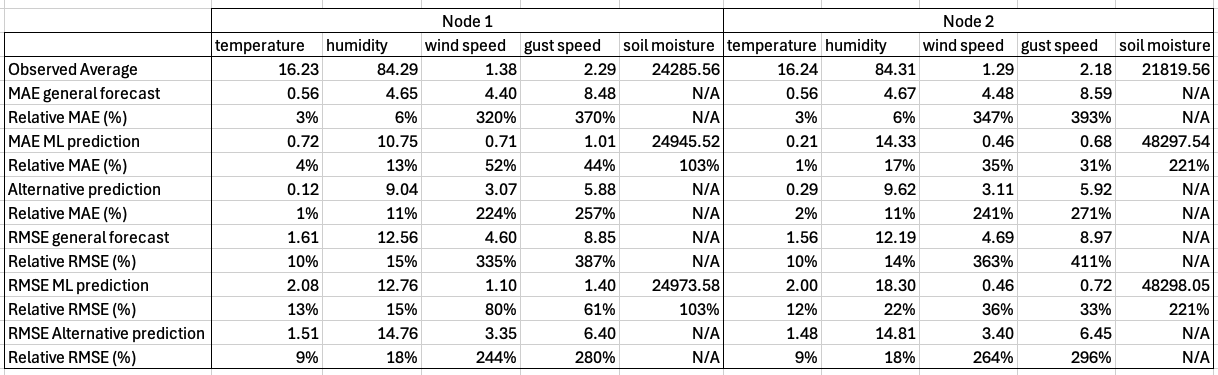
\includegraphics[width=0.9\textwidth]{contents/appendix/fig5/mae-rmse.png}
    \caption{General forecast is OpenWeather, Machine learning refers to my models, alternative refers to a mean adjusted general forecast model}
    \label{fig:mae-rmse}
\end{figure}

\begin{figure}[H]
    \centering
    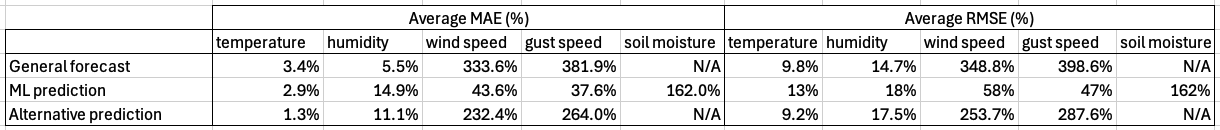
\includegraphics[width=1\textwidth]{contents/appendix/fig5/rel-mae-rmse.png}
    \caption{Table with relative MAE and RMSE averaged across node 1 and 2}
    \label{fig:rel-mae-rmse}
\end{figure}

\section{Alternative model data}\label{app:alt-data}

The below figure was used to produce the alternative model by applying these
adjustments to the general OpenWeather forecast. A positive reading means sensor
data was higher than forecast.

\begin{figure}[H]
    \centering
    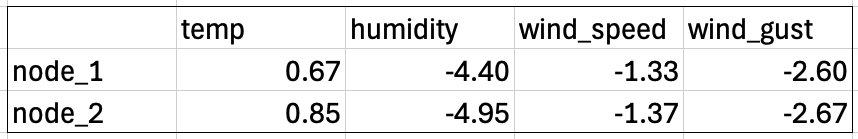
\includegraphics[width=1\textwidth]{contents/appendix/fig5/average-difference.png}
    \caption{Spreadsheet snippet showing average difference between general forecast and sensor readings between (15-27 August)}
    \label{fig:alt-data-ig}
\end{figure} 